% !TEX program = xelatex
% Main document. The heading hierarchy follows the supplied DOCX template.
\documentclass[UTF8,fontset=fandol,zihao=-4]{ctexart}
\usepackage{reportstyle}
\hypersetup{pdftitle={基于安路FPGA的双板实时图像处理系统},pdfauthor={}}
\begin{document}
\worktitle{基于安路 FPGA 的双板实时图像处理系统}
\abstractheading
本作品基于安路FPGA，设计并实现了一套集相机采集、图像处理、白细胞检测分类与实时显示于一体的双板系统。系统由PH1P35相机主板和EG4D20显示子板组成：主板负责采集和处理图像，并通过千兆以太网将视频分别发送至PC和显示子板；子板完成图像接收与缓存，通过HDMI连接显示器。系统支持$1280\times720$分辨率、30帧每秒的视频输出，将图像采集与显示终端分离，便于灵活连接和独立调试。

在图像处理方面，系统通过彩色重建、自动白平衡和自动曝光调节画面的色彩与亮度，并提供灰度、二值化、边缘、卡通、素描等多种显示模式。在白细胞识别方面，主板从完整画面中提取图像，利用量化神经网络检测白细胞位置并判断其类型，在视频中显示目标框和英文类别名称。识别结果经过跨帧确认与保持，用于减轻短时漏检和类别跳变对观察的影响。

图像处理、细胞识别及框与文字叠加均在FPGA内完成，PC上位机负责视频预览、图像保存和参数设置。用户可在运行过程中切换显示模式，调整曝光和白平衡等参数，PC与HDMI端接收相同的板端标注画面。作品形成了从相机输入到双端显示的完整处理链路，面向血涂片图像中的白细胞检测与分类，为血液细胞形态观察和血检辅助分析提供实验平台。

\section{作品概述}
\subsection{功能与特性}
系统完成$1280\times720$、30 fps相机采集、彩色重建、白平衡、自动曝光及七模式图像处理。主板将全帧图像缩放为RGB160输入，通过量化YOLO风格网络检测白细胞位置并判定五类，在视频中叠加目标框和英文类别名称。识别支路每两视频帧推理一次，中间帧保持完整结果。图像处理、检测分类、跨帧确认和标注均在FPGA完成，处理后的视频分别经网口送至PC与HDMI显示子板。

\subsection{应用领域}
作品主要面向血液细胞检测与形态学辅助分析，可用于血涂片图像的实时采集、观察、白细胞定位和分类。系统支持嗜碱性粒细胞、嗜酸性粒细胞、淋巴细胞、单核细胞和中性粒细胞五类识别，并将位置与类别直接标注在画面中，便于观察细胞形态、核对识别结果和保存典型图像。

针对血涂片观察中的照明与色彩差异，系统通过自动曝光和白平衡调节图像，并提供PC预览与HDMI显示两种观察方式，可作为血检辅助分析、血细胞形态学教学和相关检测算法验证的实验平台。

\subsection{主要技术特点}
系统在FPGA中构建流式ISP通路，完成RAW图像展开、Bayer彩色重建、白平衡、数字增益和多模式图像处理。自动白平衡根据校正前的色彩统计估计色偏，自动曝光根据校正后的亮度反馈调节曝光与增益，使图像调节与后续识别使用一致的处理链路。参数在帧边界统一生效，便于在连续视频中调整成像效果。

在模型部署方面，系统采用面向FPGA资源设计的轻量级检测分类网络，通过低位宽量化、流式首层计算和后续卷积运算单元复用，减少权重、特征存储及计算资源开销。模型直接使用ISP输出、未经风格化和文字叠加的图像，在板端完成白细胞定位、五类识别及结果确认；框与类别名称在视频发送前叠加，PC和HDMI端接收同一处理结果，无需PC参与实时推理。

\subsection{主要性能指标}
\begin{center}\small
\begin{tabularx}{\linewidth}{|L{2.5cm}|Y|}
\hline\tablehead 项目 & 指标\\\hline
图像输入 / 输出 & $1280\times720$，RAW10输入、RGB888输出，30 fps配置\\\hline
传输 / 显示 & 千兆UDP，1920包/帧；子板HDMI 720p60\\\hline
检测 / 分类 & 全帧$160\times160$ RGB输入；白细胞定位与五类识别\\\hline
推理 / 标注 & 15次/秒调度，非推理帧保持结果；目标框与英文类别名称\\\hline
模型量化 & 首尾层8位权重，中间层4位权重及激活，输入8位RGB\\\hline
整机资源 & Slice19016/21216，ERAM94/108，DSP35/40\\\hline
\end{tabularx}
\end{center}

\subsection{主要创新点}
\begin{enumerate}[label=（\arabic*）]
\item 国产FPGA内完成流式ISP与轻量级模型部署，实现白细胞检测分类和双端标注显示。
\item 抽帧推理与完整结果保持结合，按目标身份连续确认类别。
\item 统一帧身份贯穿自适应ISP、网络和显示，参数按帧提交。
\item 从数据清理、整数对拍到物理实现，以哈希关联模型与位流。
\end{enumerate}

\subsection{设计流程}
先建立采集、ISP、网络和显示链路，再接入全帧量化检测分类。WBCAtt+单一来源实验因实拍空场景误检撤回，随后使用WBCAtt+与BCCD两来源训练、量化和导出，完成整数对拍、720p调度检查、回归及物理实现后下载主板SRAM。当前工程统一收于\path{camera processing unit/}，主板、子板、训练和文档分目录管理；目录整理只调整工程引用路径，实时算法沿用最终候选实现。用户已反馈实拍改善并自行完成Flash烧录，独立定量相机验收与冷启动核验仍待完成。

\section{系统组成及功能说明}
\subsection{整体介绍}
系统由相机主板、显示子板、SC500CS 摄像头、PC 和 HDMI 显示器组成。主板采用安路 PH1P35，承担 MIPI 接收、ISP、全帧采样、量化检测分类、身份跟踪与类别确认、框与类型叠加及网络发送；子板采用 EG4D20，承担网络接收、图像重组、DDR 缓存和 HDMI 输出。ETHA 连接 PC，ETHB 镜像同一标注码流至子板。相机主链路持续前进，PC 收图速度与 CNN 忙闲不反向阻塞采集。

\begin{figure}[htbp]\centering
\begin{tikzpicture}
\node[box,text width=3.3cm] (cam) at (-3.6,0) {SC500CS 摄像头\\MIPI 2 lane RAW10};
\node[box,text width=4.4cm] (main) at (2.6,0) {相机主板 PH1P35\\采集 ISP AE AWB\\全帧量化检测分类\\框与类型叠加};
\node[box,text width=4.1cm] (pc) at (-3.6,-3.2) {PC 上位机\\原样收图 控制 存帧};
\node[box,text width=4.1cm] (sub) at (2.6,-3.2) {显示子板 EG4D20\\重组 DDR OSD HDMI};
\draw[flow] (cam)--(main);
\draw[flow] (main.south) -- ++(0,-.45) -| node[lab,pos=.55,above]{ETHA 视频} (pc.north);
\draw[flow] (main.south) -- node[lab,pos=.65,right]{ETHB 镜像} (sub.north);
\draw[ctrl] (pc.west)--(-6.3,-3.2)--(-6.3,1.6)--node[lab,above]{UDP 命令}(2.6,1.6)--(main.north);
\end{tikzpicture}
\caption{系统组成及双网口连接关系}\label{fig:system}
\end{figure}

视频使用 UDP 6000，控制使用 UDP 6001，状态与应答使用 UDP 6002。主板地址为 \code{192.168.1.66}，视频目的地址与 PC 接收地址为 \code{192.168.1.100/24}；子板在独立镜像链路上按同一目的 IP 过滤视频。子板是接收显示设备，不承担主板参数控制；因此其可达性应以接收、CRC、缓存和画面更新判断。



\lead{当前工程目录与模块边界}
项目根目录为\path{camera processing unit/}。表\ref{tab:layout}给出整理后的实际入口；下文源码路径均相对该根目录。主板工程是\path{hardware/mainboard/td_project/camera_to_dsi_display.al}，子板工程是\path{hardware/hdmi/HDMI_OUT.al}。原构建摘要保留构建时路径，不能直接当作当前磁盘位置；现存目录映射记录在\path{tools/project_layout.json}。

\begin{table}[htbp]\centering\small
\caption{当前工程的目录与职责}\label{tab:layout}
\begin{tabularx}{\linewidth}{|L{5.4cm}|Y|}
\hline\tablehead 当前目录 & 内容与作用\\\hline
\path{hardware/mainboard/} & PH1P35主板工程、相机/ISP/识别/网络RTL、工具及部署摘要\\\hline
\path{hardware/hdmi/} & EG4D20网口收流、DDR三缓冲与HDMI输出工程\\\hline
\path{yolo/wbc_bccd/} & 当前两来源训练、评估、导出及冻结资产\\\hline
\path{yolo/five/}、\path{yolo/robust/} & 当前流程复用的训练、整数参考和验证工具\\\hline
\path{docs/competition/} & 官方作品报告LaTeX、PDF及原始Word模板\\\hline
\path{docs/design_notes/} & 相机、ISP、控制、显示及检测专题资料\\\hline
\path{old/releases/}、\path{old/cellnet32/} & 历史位流与退役分类器；不代表当前活动识别方案\\\hline
\end{tabularx}
\end{table}

主板自v30起取消本地DDR至DSI显示支路并关闭7寸屏背光，视频经双网口输出；完整帧显示缓存位于子板。CellNet32与中心640/固定480分类属于历史原型。当前顶层不实例化这些分类器，但仍复用\path{classify/cvp_cell_tracks.v}和\path{classify/cvp_cell_label.v}完成身份确认和叠加；工程文件中保留的旧源码条目不等于其处于有效综合层次。\cite{repo,layout,yolortl}

数据面和控制面在主板内部汇合。图像在像素域逐拍处理，统计模块在帧尾生成亮度及色彩信息，控制器生成下一次设置；网络命令写入影子配置，再在有效帧首统一提交。帧号、配置号和图像同步标志贯穿处理链，使输出画面、状态与参数之间有明确对应关系。\cite{repo,interface}

\Needspace{10\baselineskip}
\subsection{硬件系统介绍}
\subsubsection{硬件整体介绍}
相机主板为 MLKPAI-F02，器件 PH1P35MDG324，配置 SC500CS 摄像头及两颗 YT8531 千兆 PHY。显示子板为 MLKPAI-F01，器件 EG4D20EG176，使用 YT8531 PHY 和合封 16 MB DDR1。两板以千兆网线直连，PC 连接主板另一网口，显示器连接子板 HDMI。当前主板采用网络输出结构，显示缓存位于子板。

\begin{table}[htbp]\centering\small
\caption{硬件单元与主要时钟域}
\begin{tabularx}{\linewidth}{|L{2.3cm}|L{2.6cm}|Y|}
\hline\tablehead 单元 & 时钟或规格 & 作用\\\hline
摄像头采集 & 约 40.2 MHz 组时钟 & MIPI 解包，形成 40 bit 四像素组\\\hline
主板像素处理 & 100 MHz & RAW 展开、插值、数字增益、统计、模式处理\\\hline
主板网络发送 & 125 MHz GMII & RGB 字节展开、协议发送、双口镜像\\\hline
子板接收 & 125 MHz & PHY 接收、协议解析、帧重组\\\hline
子板存储 & 150 MHz & 三缓冲、FDMA、DDR 读写\\\hline
子板显示 & 75 MHz / 375 MHz & 光栅时序 / TMDS 串化\\\hline
\end{tabularx}
\end{table}

传感器以 VTS=1003 行配置 30 fps 工作点，采窗为 $1287\times727$，有效图像为 $1280\times720$。采窗和有效输出是两个独立参数：传感器边界余量用于成像配置，下游行帧计数则严格以有效图像尺寸为准。曝光以半行为编码单位，范围为 62～1800；默认曝光码为 500，模拟增益默认档位为 108。图像输出与控制通路均围绕这一工作点设计。

\subsubsection{机械设计介绍}
机械结构采用显微镜摄像头支架V10方案，由镂空底座、排线立柱、可更换摄像头托座、遮光后盖和连接横销组成，各零件采用分件设计，便于3D打印和装配。底座用于承放开发板，立柱导槽用于整理摄像头排线；托座通过插接与横销固定，并设置间隔5 mm的三档孔位，便于粗调安装高度。

显微镜托座将摄像头固定腔与入筒段连成一体，入筒段长40 mm、外径22.75 mm，按内径23.15 mm的目镜筒设计。可拆遮光后盖采用周圈台阶限位，避让摄像头中央器件和排线接口。拔出横销后可更换竖直托座，适应显微图像采集与竖直演示两种装配方式。\cite{mechanical}

\subsubsection{电路各模块介绍}
\lead{采集与跨时钟域}
SC500CS 经 MIPI CSI-2 双通道发送 RAW10 数据。接收模块完成包解析和 RAW10 还原，\code{uial2axis} 组织行帧信息，\code{line_retimer} 将有效数据重切为每行 320 拍、每拍 4 像素，共 720 行的组流。异步 \code{group_fifo} 将采集域接入 100 MHz 主域。下游齿轮箱每次取出完整 40 bit 组，再展开为四个 10 bit 单像素，避免把组握手与单像素握手混用。

真实帧起点用于重置行列位置和像素身份。短帧或异常帧通过组数、输出像素数和流健康检查识别，尾部残留数据在新的帧身份开始前清理，避免相邻帧拼接。控制寄存器、有效标志和多位数据分别使用适合的跨域方式；整帧状态采用快照后传递，保证接收端读到同一次统计。

\lead{公共像素流}
内部接口以 \code{valid} 配合固定 128 bit 像素字传递，不设置摄像头反压。RGB 为 24 bit，坐标各 12 bit，帧身份为 32 bit，配置号为 16 bit，模式号为 8 bit，另携带 SOF/EOL/EOF、错误与工作状态。每帧应有 $1280\times720=921600$ 个有效像素、720 个行尾和 1 个帧尾。

\begin{table}[htbp]\centering\small
\caption{公共像素字的关键字段}
\begin{tabularx}{\linewidth}{|L{3.1cm}|Y|}
\hline\tablehead 位范围 & 含义\\\hline
23:0 & RGB888，R 为高字节\\\hline
35:24 / 47:36 & 零起始 x / y 坐标\\\hline
79:48 / 95:80 & 采集帧身份 / 生效配置号\\\hline
103:96 & 图像模式号\\\hline
104 / 105 / 106 & SOF / EOL / EOF，与对应像素同拍\\\hline
107～111 & 错误、OSD、AE、WB 状态\\\hline
127:112 & 预留字段\\\hline
\end{tabularx}
\end{table}

点运算须对 RGB 和整个元数据施加相同延迟；窗口运算的输出坐标必须描述实际窗口中心。窗口边界需要补齐首末行列，并在帧结束时排空流水。分类支路使用未经过对比度、风格化和 OSD 的 \code{clean_pixel}，避免展示效果改变算法输入分布。\cite{interface}

\lead{网络发送与带宽}
四个 RGB888 像素合并为 96 bit 组，经跨域缓存进入 125 MHz 发送域，再按 R、G、B 顺序展开。每个 UDP 包的应用头为 6 B：1 B 帧序号、1 B 格式和 4 B 大端字节偏移，随后为 1440 B 图像数据，即 480 个像素。帧内偏移由源数据描述符提供，与真实帧身份一致。
\begin{align}
B_{\rm frame}&=1280\times720\times3=2764800\ \mathrm{B},\\
N_{\rm packet}&=2764800/1440=1920.
\end{align}
以太网头、IP 头、UDP 头、应用头和 FCS 合计 60 B，因此每个以太网帧为 1500 B。计入 8 B 前导码与 12 B 帧间隙，30 fps 时预算为
\begin{equation}
R_{\rm wire}=1920\times(1500+8+12)\times8\times30
 \approx700.4\ \mathrm{Mb/s}.
\end{equation}
相应单帧线时约 23.35 ms，小于 33.33 ms 帧周期。两颗 PHY 各自完成千兆协商，ETHB 复制主发送流；PC 与子板在各自物理链路上接收，因此无需在同一链路上重复发送两份视频。

\lead{子板重组与显存写入}
协议栈输出按包连续到达的 UDP 载荷，帧缓存需要按光栅顺序排列的固定长视频。\code{cvp_rx_assemble} 解析应用头，以暂存 FIFO 保存字节，以描述符保存目标偏移。输入端检查格式、界限、对齐和顺序；输出端先填充缺口，再输出本包像素，帧尾补齐到规定长度。

小缺口白名单为 0～4 个完整图像包；缺口超限、重复或逆序的数据不会破坏已提交的光栅位置，接收端跟踪丢弃并在合法新帧起点恢复。填充阶段受缓存水位约束时，合法包可推进已承诺位置而不进入载荷队列，防止输入位置停滞导致后续缺口级联。链路断开、锁相异常与错误恢复分别经过同步和复位时序控制。

写侧 FIFO 必须积累完整 DMA 突发的数据后才提出请求，256 字突发的门槛与原生 FIFO 标志语义一致。补洞和补帧输出限制为每三拍一个像素，以匹配写通路可持续吞吐；发出下一帧同步前须等待本帧 DMA 写入完成，而不能仅凭重组器已经输出最后一个像素判断帧结束。\cite{hdmistart,hdmicolor}

\lead{DDR 读出与显示}
DDR1 按 4 MB 帧步进分配三块缓存，总计 12 MB。写侧以 30 fps 提交帧，读侧以 60 Hz 输出；只有完整写入的缓存才可发布，显示端在 VS 边界切换，避免读写使用同一帧槽。首帧就绪前输出黑底，读空时屏蔽该场余下视频，避免把失去位置关系的旧像素持续送往 HDMI。

按显存侧 32 bit 像素字计算，写与读的带宽为
\begin{equation}
B_{\rm DDR}=1280\times720\times4\times(30+60)
 =331.776\ \mathrm{MB/s},
\end{equation}
约为 600 MB/s 峰值的 55.3\%。预算还需结合仲裁、行预取、刷新和总线停顿验证，不能将峰值余量直接等同于任意停顿均可承受。

DDR 返回数据以 DQS 为采样基准，在上升沿采集低 16 bit、下降沿拼接完整 32 bit 字，再用 Gray 指针异步 FIFO 交给控制器域。数据有效由真实采集产生，避免使用固定请求延迟推断。控制器执行周期刷新并保证初始化及 DLL 稳定等待。显示端对齐 FIFO 读延迟，将 RGB、DE、HS、VS 延迟一致后送往 TMDS 编码器；OSD 在相同光栅坐标下叠加。\cite{hdmicolor}

\Needspace{10\baselineskip}
\subsection{软件系统介绍}
\subsubsection{软件整体介绍}
软件包括FPGA RTL、离线训练与整数导出、PC收图控制程序及验证脚本。当前顶层\path{hardware/mainboard/user_source/hdl_source/design_top_wrapper.v}将\code{cvp_advanced}的clean RGB送入\code{cvp_yolo160_detector}，后接\code{cvp_yolo_tracks}与\code{cvp_cell_label}；标注后RGB进入\code{pack_4}及网络发送。活动识别支路参数为\code{FRAME_INTERVAL=2}、\code{SINGLE_TARGET=1}、\code{FULL_NAMES=1}。PC GUI入口位于\path{hardware/mainboard/tools/cam_gui_v27.py}，仅负责原样预览、存帧与参数控制，实时识别和叠加均在FPGA完成。

上位机使用独立请求号管理事务。SET 写入影子寄存器，COMMIT 请求在下一有效帧首生效，状态返回接受、待生效、生效、忙或拒绝。客户端等待应答并重试，提交后查询实际值，未核对通过不显示成功。传感器应答表示写入事务完成，光学曝光变化仍需等待传感器输出反映新参数。

\begin{figure}[htbp]\centering
\begin{tikzpicture}
\node[box,text width=3.0cm] (a) at (-4.3,0) {采集与去马赛克\\校正前 RGB};
\node[box,text width=3.4cm] (b) at (0,0) {白平衡与数字增益\\标准 clean RGB};
\node[box,text width=2.8cm] (c) at (4.4,0) {色阶与七模式\\框 类型 UDP};
\node[box,text width=5.0cm] (awb) at (-3.3,-2.6) {AWB 校正前色彩统计\\中性样本 → R/B 增益};
\node[box,text width=5.0cm] (ae) at (3.3,-2.6) {AE 校正后亮度统计\\PID → 曝光与数字增益};
\draw[flow] (a)--(b);\draw[flow] (b)--(c);
\draw[ctrl] (a.south) -- ++(0,-.4) -| (awb.north);
\draw[ctrl] (awb.east) -- ++(.4,0) |- (b.south west);
\draw[ctrl] (b.south) -- ++(0,-.45) -| (ae.north);
\draw[ctrl] (ae.east)--++(.5,0)|- (0,1.6)--(b.north);
\end{tikzpicture}
\caption{主板像素通路与自动图像调节的统计口径}\label{fig:isp}
\end{figure}

图像接收线程和状态线程分别处理 UDP 6000 与 6002，GUI 定时取得线程快照并更新画面。单帧按帧序号和字节偏移拼接，状态区结合 RAW 组数、输出长度、帧率及累计错误观察链路。一次接收程序独占视频端口，避免多个进程分流同一批 UDP 包。

\Needspace{10\baselineskip}
\subsubsection{软件各模块介绍}
\lead{RAW 与彩色重建}
RAW10 展开后先经过四拍相位保持延迟，再进入 $3\times3$ Bayer 双线性插值。当前 RAW 通路不执行坏点替换。行列计数以有效帧起点对齐，并以 BGGR 相位选择 R、G、B 的重建位置。以蓝色中心 $p_{11}$ 为例，
\begin{align}
\widehat B&=p_{11},\\
\widehat G&=(p_{01}+p_{10}+p_{12}+p_{21})/4,\\
\widehat R&=(p_{00}+p_{02}+p_{20}+p_{22})/4.
\end{align}
红色中心的 R/B 关系对换；绿色中心根据所在行，从水平和垂直的同色邻点分别求均值。插值结果取高 8 bit 形成 RGB888。Bayer 不同位置的邻点颜色不同，任何 RAW 空间处理都必须根据采样相位选择邻域，不能把几何相邻直接当作同色。\cite{rtl}

\lead{白平衡与数字增益}
四种白平衡模式为标定预设、色温 K 值、手动 RGB 和自动场景。预设为 R344/G256/B451，Q8 中 256 表示 1 倍。设白平衡编码为 $w_c$，全局数字增益编码为 $d$，两者先相乘再统一校正：
\begin{align}
g_c&=\left\lfloor(w_c d+128)/256\right\rfloor,\\
O_c&=\min\!\left(255,\left\lfloor(I_cg_c+128)/256\right\rfloor\right).
\end{align}
此结构只在最终 RGB8 输出处饱和，避免先对白平衡结果截断，再乘全局增益造成中间精度损失。$g_c$ 在帧首锁存，整帧使用同一组通道设置。

AWB 使用数字校正前的 RGB 估计原始色偏。先以标定先验拉平色度，筛选不接近黑位和削顶、通道差异足够小的中性样本；保守判据要求归一色度范围不超过最大通道的 $1/8$。全画面分为四个象限，至少两个象限具有足够样本才接收估计，避免单一物体主导白平衡。

对中性集合 $\mathcal N$，候选增益以绿色为锚点：
\begin{equation}
w_R^{\rm cand}=\operatorname{clip}_{128}^{1024}
\left(256\frac{\sum_{p\in\mathcal N}G_p}{\sum_{p\in\mathcal N}R_p}\right),\qquad
w_B^{\rm cand}=\operatorname{clip}_{128}^{1024}
\left(256\frac{\sum_{p\in\mathcal N}G_p}{\sum_{p\in\mathcal N}B_p}\right).
\end{equation}
候选值先限制在标定增益的 $\pm25\%$ 邻域，与标定基准按置信度混合，再通过 $1/16$ 权重的一阶平滑更新。全帧样本数、有效象限或通道和不满足条件时冻结增益，并输出原因与样本状态。

\lead{亮度统计与高光保护}
AE 统计位于白平衡与全局增益之后、风格化之前。单像素亮度及高光比例为
\begin{equation}
Y=\left\lfloor\frac{77R+150G+29B+128}{256}\right\rfloor,\qquad
r_{\rm clip}=\frac{\#\{Y\ge245\}}{N}.
\end{equation}
默认目标亮度为 112，死区为目标 $\pm8$。当高光比例超过 5\% 时，控制器可降低实际目标，在 32～112 范围内保留高光安全裕量，避免高反差场景反复“保护高光”和“恢复固定均值”。GUI 同时显示实际目标，均值低于 112 不必然代表尚未收敛。

\lead{自适应采样与定点 PID}
控制器在帧事件上决策。亮度误差绝对值至少为 24 时使用两帧平均，接近目标时使用四帧平均；两种窗口都保留四分之一亮度码精度。设窗口均值的 Q2 编码为 $M_k$，目标 Q2 编码为 $T_k$，则
\begin{align}
e_k&=T_k-M_k,\\
I_k&=\operatorname{clip}_{-512}^{512}(I_{k-1}+e_k),\\
D_k&=(D_{k-1}+M_{k-1}-M_k)\mathbin{\gg}1,\\
C_k&=(6e_k+3I_k+D_k)\mathbin{\gg}2.
\end{align}
$K_p,K_i,K_d$ 的 Q10 编码分别为 6、3、1，实际系数为 $6/1024$、$3/1024$、$1/1024$。上式右移 2 位消除测量 Q2 倍率；$C_k$ 随后作为 Q10 比例调节量参与总曝光更新。微分使用测量变化，目标变化不会直接引入微分冲击；误差反向时清除旧积分和微分历史。

控制量与误差方向相反时取零，大误差比例步长限幅为 $256/1024$，小误差为 $64/1024$；饱和时抑制继续积分。在死区内停止调节并清理历史。令 $U_k=E_kd_k$ 为“曝光半行码×Q8 数字增益”的整数总曝光量，
\begin{align}
\Delta U_k&=\max\!\left(256,\left\lfloor\frac{U_k|C_k|+512}{1024}\right\rfloor\right),\\
U_{k+1}&=\operatorname{clip}_{62\times256}^{1800\times1024}
\bigl(U_k+\operatorname{sgn}(C_k)\Delta U_k\bigr)\qquad(C_k\ne0).
\end{align}
先把 $U_{k+1}$ 分配给传感器曝光：当 $U_{k+1}\le1800\times256$ 时令数字增益为 1 倍，曝光由 $U/256$ 四舍五入得到；超过该值则固定曝光 1800，再由 $U/1800$ 得到 1～4 倍数字增益。AE 不自动改变模拟增益，模拟增益保留用户设定。

计算按测量、历史更新、乘加、限幅、总量更新和执行器分配分段，避免把整条 PID 算术路径集中在一拍。除以常数 1800 使用移位恢复除法，利用帧间充足时间降低组合逻辑压力。\cite{pid}

\lead{参数执行与一致性}
传感器桥保持一次仅有一个在途事务，曝光寄存器以 group hold 成组提交，I2C NACK 或超时通过状态返回。涉及曝光变化的提交确认后，丢弃两帧旧反馈再重新统计；纯 FPGA 数字增益在 SOF 原子提交后即可统计新数据，不增加额外两帧等待。控制器仅在实际生效参数与请求匹配时保存对应 PID 历史，手动请求优先并使旧历史失效。

\lead{七种实时图像模式}
七种模式的选择与处理方式见下表。

\begin{table}[htbp]\centering\small
\caption{图像模式及运算原理}
\begin{tabularx}{\linewidth}{|L{.9cm}|L{1.8cm}|Y|}
\hline\tablehead 编号 & 模式 & 实现\\\hline
0 & 原图 & 标准校正图像直通\\\hline
1 & 灰度 & $Y=(R+2G+B)\gg2$，三通道同值\\\hline
2 & 二值化 & 灰度与可配置阈值比较\\\hline
3 & Sobel 边缘 & 窗口梯度、高低门限与连通判决\\\hline
4 & 卡通 & 中值平滑、每通道 3 bit 量化、轮廓描边\\\hline
5 & 素描 & 白底黑线；独立阈值和线宽\\\hline
6 & 复古暖色 & 定点 sepia 矩阵映射与饱和限幅\\\hline
\end{tabularx}
\end{table}
Sobel 在灰度 $3\times3$ 窗口中计算水平和垂直梯度，以 $|G_x|+|G_y|$ 近似幅值，避免平方根。边缘与素描分别保存阈值与线宽，低阈值可联动为高阈值的一半，参数通过帧首提交保持一帧内一致。卡通先保边平滑，再降低颜色级数，最后叠加轮廓。

显示色阶根据 32 箱亮度直方图选取黑白分位点，用限幅线性映射拉伸对比度；低跨度画面旁路，增益限定在 0.5～2 倍。它属于自动色阶，不等同于使用整条累计分布函数的直方图均衡。算法支路可直接使用处理前的标准像素流。


\lead{全帧采样与网络结构}
\code{cvp_yolo160_detector} 从 $1280\times720$ clean RGB 直接采样为 $160\times160$，覆盖全画面，不再受中心640或固定480窗口限制。采样位置为
\begin{equation}
x_k=4+8k,\qquad y_j=2+4j+\lfloor j/2\rfloor,\qquad k,j=0,\ldots,159.
\end{equation}
这是横纵不同比例的直接近邻缩放，没有补边。检测框解码后按横向8倍、纵向4.5倍恢复至原画面，并裁到合法边界；训练与整数参考使用一致的坐标约定。小目标在160输入中损失细节，需要真实相机验证。

本网络是自行实现、面向RTL的单尺度YOLO风格检测器，采用锚框、objectness和类别联合预测；并非官方YOLOv5/v8完整移植，不具有其多尺度颈部与检测头。十层普通卷积的输出通道为8/8/8/16/24/40/80/24/40/30，前四层后各有 $2\times2$ 最大池化；第八层为 $1\times1$，其余为 $3\times3$，最后空间尺寸为 $10\times10$。

\begin{table}[htbp]\centering\small
\caption{板端检测网络的空间尺寸与通道}
\begin{tabularx}{\linewidth}{|L{1.8cm}|L{3.0cm}|L{2.4cm}|Y|}
\hline\tablehead 层 & 输入空间 / 通道 & 输出通道 & 输出空间与处理\\\hline
1 & $160^2$/3 & 8 & $80^2$，卷积后池化\\\hline
2 & $80^2$/8 & 8 & $40^2$，卷积后池化\\\hline
3 & $40^2$/8 & 8 & $20^2$，卷积后池化\\\hline
4 & $20^2$/8 & 16 & $10^2$，卷积后池化\\\hline
5 / 6 / 7 & $10^2$/16、24、40 & 24、40、80 & $10^2$，$3\times3$卷积\\\hline
8 / 9 & $10^2$/80、24 & 24、40 & $1\times1$ / $3\times3$卷积\\\hline
10 & $10^2$/40 & 30 & 三锚框各10字段\\\hline
\end{tabularx}
\end{table}

每个格点的三个锚框各输出 $t_x,t_y,t_w,t_h,t_o$ 和五类logit，共30通道、3000个有符号整数输出。160尺度锚框为 $(20,24),(40,48),(80,88)$。设格点坐标为 $(g_x,g_y)$、步长16、锚框宽高为 $(a_w,a_h)$，浮点解码为
\begin{align}
(c_x,c_y)&=16\,[2\sigma(t_{x,y})-0.5+(g_x,g_y)],\\
(w,h)&=[2\sigma(t_{w,h})]^2\,(a_w,a_h),\\
s&=255\,Q_{\sigma}(t_o),\quad \widehat c=\arg\max_c t_c.
\end{align}
硬件使用ROM sigmoid、整数运算及边界限幅，按相同整数参考逐项核对，不直接在FPGA计算指数。\cite{yolortl,twosource}

\lead{量化计算与调度}
首层输入为8 bit RGB、权重8 bit；中间卷积权重有符号4 bit、激活无符号4 bit；末层权重8 bit，输出有符号16 bit logit。训练先浮点再折叠BatchNorm，按输出通道导出偏置和移位，量化感知前向使用float64精确整数累加，避免半LSB附近与RTL舍入不同。

\code{yolo160_first} 在采样流上计算首层并池化，不缓存整张RGB输入。\code{yolo160_core} 对后九层采用四输出通道复用同一输入激活，特征在片内RAM间交替读写，4 bit激活打包存储；低位宽乘法采用LUT移位加法结构。四路是硬件并行度，不是把模型改成分组卷积。首层累加界限按有符号32 bit、后续按24 bit导出检查，ROM与元参数均带哈希。

默认 \code{FRAME_INTERVAL=2}：相机按30 fps配置，网络15次/秒调度。一次720p节拍联合仿真从采样起点到检测提交为6295080拍，100 MHz下62.9508 ms，小于66.67 ms；不等于实测曝光至屏幕延迟。网络忙闲不反压相机，配置改变或不完整输入按事务中止，不发布半成品结果。\cite{yoloreport}

\begin{figure}[htbp]\centering
\begin{tikzpicture}
\node[box,text width=10.7cm] (a) at (0,0) {全帧clean RGB $1280\times720$ 与帧号、配置号\\每两帧采样一次RGB160};
\node[box,text width=10.7cm] (b) at (0,-1.7) {流式首层与四路复用卷积\\$10\times10$格点、三锚框、五类联合输出};
\node[box,text width=10.7cm] (c) at (0,-3.4) {整数解码、top20、NMS、身份匹配与类别确认\\非推理帧保持完整结果，最多选择一个细胞};
\node[box,text width=10.7cm] (d) at (0,-5.1) {框左上角英文全称，视频帧首锁存\\标注RGB经双网口送往PC与HDMI子板};
\draw[flow] (a)--(b);\draw[flow] (b)--(c);\draw[flow] (c)--(d);
\end{tikzpicture}
\caption{全帧联合检测分类与单框保持的主板实现}\label{fig:yolo}
\end{figure}

\lead{候选筛选、跨帧保持与英文全称}
\code{yolo160_boxes} 使用整数sigmoid查表值 $Q_{\sigma}\in[0,255]$，检测分数为其objectness值乘255，五类logit的argmax独立决定类型。当前阈值52020/65025，由公开验证与用户开发截图联合校准；检测分数与五类判断解耦，使只有定位监督的BCCD样本不因类别分数乘积被再次过滤。这些分数不是经概率校准的正确率。按分数稳定排序保留top20，再执行跨类别NMS，IoU阈值103/256，最多提交五个候选。候选均来自同一次网络推理，各自带框与类别，不把一个固定视场的分类标签复制到其他框。

\code{cvp_yolo_tracks} 进行几何身份匹配，每个目标首次连续两次结果一致才确认，切换类别需连续三次异类一致。优先维持已选中身份，失去该身份后才选最近画面中心的有效目标；距离比较分拍执行。每帧最多显示一个框。跳过推理的帧保持最近完整结果；连续一、两次推理漏检保留身份、框和类别，第三次仍漏检撤框。框有效期5个视频帧，类别有效期15帧；配置变化、超时或非法帧身份拒绝旧结果。WAIT表示尚未确认或失效，不是训练类别。

匹配、类别投票和目标选择全部结束才原子发布，\code{cvp_cell_label} 在显示帧首锁存，更新过程中不临时清空。文字区域为160×16像素，框左上角显示 Basophil、Eosinophil、Lymphocyte、Monocyte、Neutrophil；顶部或右侧空间不足时限制在屏内。SW1控制标注显隐，标注在主板打包和双网口分流之前完成。连续确认能抑制孤立跳变，也会增加切换等待；持续错误类别仍可能被确认。\cite{yoloreport}

\lead{上位机函数与协议}
上位机主要入口及输入输出关系见下表。

\begin{table}[htbp]\centering\small
\caption{上位机主要入口与数据关系}
\begin{tabularx}{\linewidth}{|L{3.5cm}|Y|}
\hline\tablehead 入口 & 输入和输出\\\hline
\code{mode_changed} & 输入所选模式，切换参数面板并提交模式设置\\\hline
\code{edge_changed} & 输入阈值、线宽和联动状态，校验并更新模式参数\\\hline
\code{send_thresholds} & 合并连续滑动事件，提交当前模式参数\\\hline
\code{submit} / \code{snapshot} & 提交请求 / 读取控制线程状态快照\\\hline
\code{update} & 获取图像和状态，刷新预览、确认值与错误信息\\\hline
\end{tabularx}
\end{table}
命令解析在 RGMII 接收侧检查以太类型、IPv4/UDP、端口和魔数；命令事件跨域进入配置控制器。16 B 控制包携带魔数、请求号、配置号、操作码、地址和 32 bit 参数，均采用大端编码。SET、COMMIT、GET 和时间同步各有明确语义，配置应答与视频状态经 UDP 6002 返回。




\begin{figure}[htbp]\centering
\begin{tikzpicture}
\node[box,text width=10.7cm] (a) at (0,0) {CSI-2 RAW10 → 行帧规整 / 异步FIFO → Bayer插值};
\node[box,text width=10.7cm] (b) at (0,-1.45) {\code{cvp_advanced}：白平衡 / 数字增益 → clean RGB\\校正前色彩统计用于AWB，校正后亮度统计用于AE};
\node[box,text width=4.6cm] (v) at (-3,-3.65) {视频主路：七模式\\持续输出720p30 RGB};
\node[box,text width=4.6cm] (y) at (3,-3.65) {识别支路：全帧RGB160\\15 Hz检测 / 分类 / 跟踪};
\node[box,text width=10.7cm] (o) at (0,-5.9) {帧首锁存完整结果 → 单框与英文全称叠加\\四像素打包 → 跨域 → ETHA / ETHB镜像};
\draw[flow] (a)--(b);
\draw[flow] (b.south) -- ++(0,-.3) -| (v.north);
\draw[flow] (b.south) -- ++(0,-.3) -| (y.north);
\draw[flow] (v.south) -- ++(0,-.35) -| (o.north west);
\draw[ctrl] (y.south) -- ++(0,-.35) -| (o.north east);
\end{tikzpicture}
\caption{当前主板视频与识别并行通路，虚线传递框和类别结果}
\end{figure}

\lead{模型资产与部署绑定}
活动权重位于\path{hardware/mainboard/user_source/hdl_source/yolo/model/}，\path{active_model.json}记录模型身份与ROM哈希。训练冻结资产位于\path{yolo/wbc_bccd/frozen/}，包括量化权重、数据审计、阈值协议与工程试验策略。最终候选bit和物理摘要位于\path{hardware/mainboard/reports/yolo_wbc_bccd15/current/physical/}，部署状态位于\path{hardware/mainboard/deployment_state.json}。\path{source_hashes.json}中的历史路径通过目录映射定位，不能因移动文件夹而改写历史构建记录。\cite{layout,twosource}

\lead{结果接口与数据身份}
检测支路携带采样源帧号、配置号和全画面坐标，候选提交由独立commit事件标识。跟踪器拒绝重复、过迟、未来或配置不一致的结果，显示取完整快照。原公共图块桥保留扩展能力，但当前有效网络支路不经过固定ROI图块或CellNet装载器。

诊断结果邮箱携带帧号、目标标识、确认类别、包围框和时间戳，接收背压不阻塞板端确认。PC不依据诊断包补画。背景负样本通过objectness损失训练拒识，没有第六个背景类型；低分候选被阈值删除。无检测、尚未确认与五类有效结果具有不同控制语义。\cite{interface,yolortl}

\section{完成情况及性能参数}
\subsection{整体介绍}
基础相机、网络及HDMI显示链路已有历史实板记录。当前两来源模型完成整数参考、RTL、720p视频调度和物理实现检查，于2026年10月21日11:37由TD6.2成功下载PH1P35MDG324主板SRAM。用户随后反馈实拍效果较前版更好，并表示已自行完成Flash烧录；此反馈属于定性实板观察，尚无带标签相机数据的独立定量准确率、当前HDMI验收或断电冷启动记录。

当前主工程位于camera processing unit目录。活动硬件树为\path{hardware/mainboard/}和\path{hardware/hdmi/}。整理前构建使用既有主板工程，构建时.al哈希保存在冻结资产；整理后.al中的文件路径已随目录调整，因此不再把当前工程文件写成“字节不变”。最终候选bit、模型和非路径源码的身份由清单核对；历史构建路径与当前位置通过映射关联。旧bit、源码和模型仍在\path{yolo/wbc_bccd/baseline/}保留。

\Needspace{10\baselineskip}
\subsection{工程成果}
\subsubsection{机械成果}
完成显微镜摄像头支架V10的三维设计，形成显微镜采集与竖直演示两套装配模型，提供六种零件的可编辑模型及STL打印文件。底座、立柱与托座实现开发板承放、排线整理和摄像头定位；遮光后盖采用一体式周圈台阶结构。已完成模型闭合性、几何配合和STL检查，打印后的承载、遮光及合焦效果需结合实物试装确认。\cite{mechanical}

\subsubsection{电路成果}
主板形成 MIPI 接收、RAW10 解包、ISP、PID 曝光控制、全帧RGB160采样、量化联合检测分类、单目标身份与类别确认、框与类型叠加、双口发送和网络命令通路；子板维持协议接收、帧重组、三缓冲显存、DQS 读回与 HDMI 通路。本轮资源与时序统计包含整个主板，不是独立 CNN 核的综合估计。

\begin{table}[htbp]\centering\small
\caption{当前两来源模型位流的完整布线资源与时序}
\begin{tabularx}{\linewidth}{|L{3.2cm}|Y|}
\hline\tablehead 指标 & 当前实现结果\\\hline
Slice & 19016/21216，89.63\%\\\hline
ERAM20K & 94/108，87.04\%\\\hline
DSP & 35/40，87.50\%\\\hline
setup WNS & +0.102 ns\\\hline
hold WNS & +0.020 ns\\\hline
时序结论范围 & 既有约束下的最终物理实现摘要\\\hline
\end{tabularx}\label{tab:resource}
\end{table}

主板采用PH1P35MDG324，工具为TD 6.2.168116；像素处理与推理为100 MHz，GMII发送为125 MHz。表\ref{tab:resource}依据当前保留的\code{build_result.json}与发布摘要，Slice剩2200个，ERAM剩14块，DSP剩5个。原始\code{route.area}、\code{route.timing}及部分运行日志已在目录整理时清理，本文不将其列为现存可复查文件。摘要中的正裕量表示既有约束下的静态时序通过，新增网络或修改路径仍需重新实现。\cite{resource,timing}

子板沿用已有显示工程，RGMII采样、DDR控制、显示像素时钟与串化时钟在约束中显式组织，异步传递由同步器或FIFO完成。本次作品报告更新未重新构建或下载子板；其验证结果按历史资料解释。\cite{hdmicolor}

\subsubsection{软件成果}
PC GUI 支持原样收图、完整 RGB 帧保存、七模式切换、轮廓参数与白平衡控制。实时细胞检测、取图、分类和文字不在 PC 运行，视频内的框和类型来自主板 RGB；通信统计位于图像外。控制参数以请求、应答、提交和查询组成事务，界面显示确认值；接收线程与状态线程独立运行，避免控件操作阻塞收图。

离线工具完成掩膜转整细胞框、去重与负样本生成、模型训练、量化感知训练、ROM 导出、整数参考推理、网络向量生成及 RTL 记分板检查。训练与评估在开发电脑执行，不参与相机实时推理链路。构建与下载记录核验源码、模型和bit哈希，已核实的成功记录为PH1P35主板SRAM下载。后续本机自动Flash操作校验失败，用户自行烧录成功的反馈另行记录；本轮未重新下载HDMI子板。\cite{gui,interface,training}

\Needspace{9\baselineskip}
\subsection{特性成果}
\lead{图像与自动调节功能}
上板系统提供 720p30 图像输出，七种模式可运行时切换；白平衡支持预设、色温、手动和自动模式；AE 使用曝光优先的 PID 和全局数字增益。图像模式、白平衡与数字增益在帧边界提交，曝光设置通过传感器事务执行。上位机显示实际目标、设置确认和链路健康，便于区分用户设置、已提交状态及图像反馈。

控制模型对明暗场、数字增益分配、高反差、交替亮度和确认延迟进行检查。两帧与四帧窗口切换受误差阈值控制；达到死区后停止调节，失败事务后重新收集统计。已有完整视频 RTL 用例覆盖 460 帧，核对帧身份、长度、非黑输出与流健康；这些属于模型和仿真检查，不能代替本轮新权重位流的相机实拍结论。\cite{pid}

\lead{网络与显存一致性}
既有发布摘要记录主板42项RTL、两组完整网络包校验和38项Python测试通过。本次仅更新报告，未重跑这些硬件回归。网络包由独立 CRC/IP/UDP 校验器解析，避免发送端与检查端共用同一错误计算过程。历史子板验证从GMII/RGMII输入到重组、DMA、DDR引脚和HDMI编码器前RGB分层核对，验证范围延伸到实际数据显示的位置。

\begin{table}[htbp]\centering\small
\caption{子板显示链路的历史量化验证（本次未重跑）}
\begin{tabularx}{\linewidth}{|L{3.1cm}|Y|}
\hline\tablehead 检查对象 & 结果及条件\\\hline
协议与重组 & 历史8场景回归通过，覆盖完整帧、丢包、重复、乱序和坏FCS等\\\hline
全分辨率工况 & 历史1920包/帧、11帧向量逐字节核对\\\hline
仲裁与刷新压力 & 历史压力扫描包含2 ms总线黑窗注入\\\hline
OSD落点 & 历史账本逐像素diff=0，图案与logo区域分别核对\\\hline
本次范围 & 核对现存文档与源码；未重跑子板仿真或重新上板\\\hline
\end{tabularx}
\end{table}

表中结果来自保留的子板专题文档，反映当时的回归记录。协议和像素仿真不覆盖板上全部电气采样裕量，实际工作还依赖RGMII采样相位、DDR引脚约束、布线和供电条件。\cite{hdmicolor}


\lead{联合检测分类的整数与视频验证}
本轮两来源模型接入的14张自然图及派生负图覆盖全部五类输出。每张逐项核对十层整数输出、6400个首层特征字、3000个logit和最终框、类型、分数，与独立整数参考完全一致。五项组件测试覆盖全帧采样与抽帧、top20与NMS、身份与类别确认、单目标选择及英文全称；三项既有跟踪回归包括90帧五目标参考策略。英文全称边缘位置和17941个文字像素有单独核对。

两种完整720p30时序各输入六帧，分别使用突发输入与每像素三拍、每行4444拍的输入节拍，验证15 Hz支路完成三次检测，非推理帧保持结果。第3至6帧有边框，第5至6帧有确认后的类别文字，更新中没有临时清空框。组件另测两次漏检保留、第三次撤框、配置切换、超时及重新出现确认。最慢节拍从采样起点到提交6295080拍，约62.95 ms。仿真证明数值与调度，不等同相机实测15 Hz或实拍零闪烁。42项原视频RTL、两项包完整性及38项Python回归均重新通过。\cite{yoloreport}

\lead{历史方案与当前报告范围}
早期CellNet32与中心窗口分类、单WBCAtt+实验均属于历史方案。单来源模型曾在同源公开TEST获得92.39\%联合macro-F1，但出现实拍空场景误检并被撤回；该结果不能写作当前部署成绩。当前模型是\code{wbc_bccd160_devcam_20261021}，采用两来源训练及新的objectness评分。下文只以当前冻结资产统计数据与模型表现，历史失败用于说明引入真实背景域和开发校准的原因。\cite{repo,twosource}

\lead{两来源数据与质量控制}
WBCAtt+以整细胞掩膜外接框提供五类和定位监督；BCCD仅提供白细胞定位监督，类别保持-1并屏蔽分类损失。原图和派生背景裁图数量分别统计，派生图继承父图划分。解码RGB160跨划分精确重复为零，但没有患者级独立性证明；TEST在前期实验中已查看，本轮只作为已使用测试集回归。\cite{wbcatt,datarepo,training}

\begin{table}[htbp]\centering\small
\caption{当前模型冻结数据划分（原图 / 派生负裁图）}
\begin{tabularx}{\linewidth}{|L{2.2cm}|Y|Y|}
\hline\tablehead 划分 & WBCAtt+ & BCCD\\\hline
TRAIN & 6021 / 6020 & 205 / 270\\\hline
VAL & 1010 / 1010 & 87 / 122\\\hline
已使用TEST & 3017 / 3017 & 72 / 99\\\hline
\end{tabularx}
\end{table}

\begin{center}
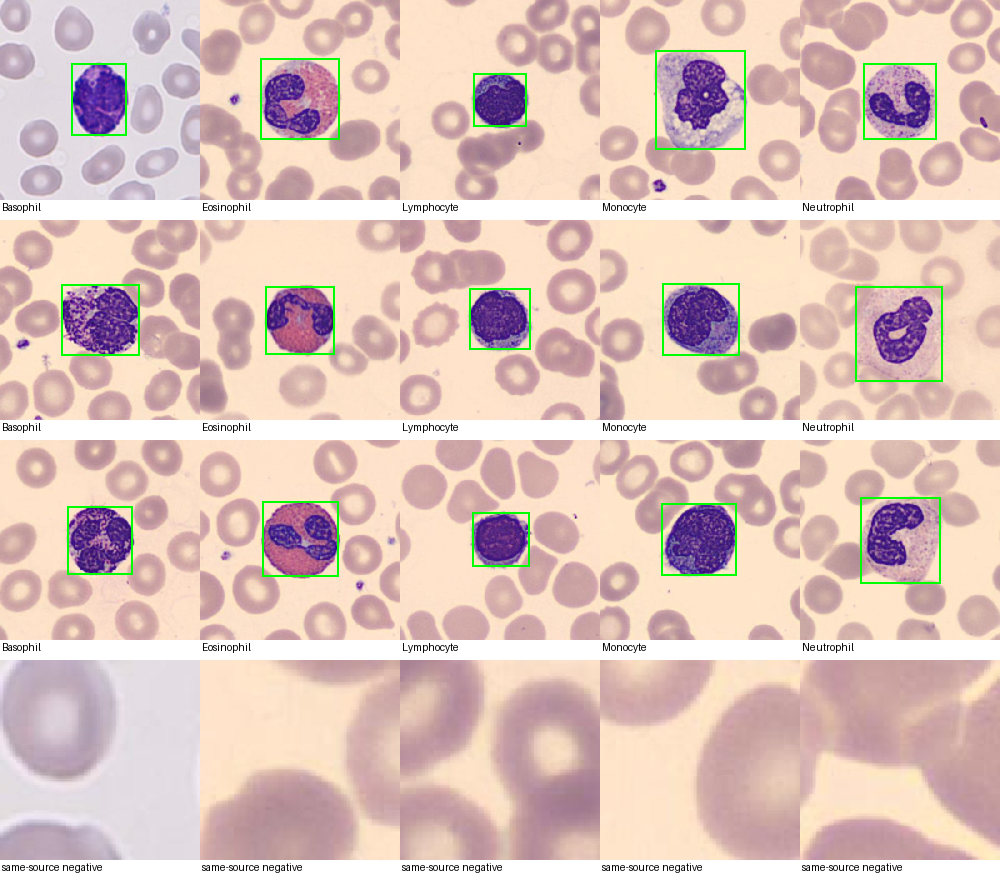
\includegraphics[width=0.82\linewidth]{images/wbcatt_training_preview.png}
\captionof{figure}{仅取TRAIN的五类标注与同源负裁图示例；绿色框来自整细胞掩膜，不是网络预测或主板实拍。}
\end{center}

\lead{WBCAtt+与BCCD两来源重训及当前部署}
本轮仅使用两套采集数据，不加入Raabin图像或Raabin训练权重。初始化来自从随机权重开始的WBCAtt-only FP32 checkpoint。WBCAtt+的TRAIN/VAL/TEST原图为6021/1010/3017，派生背景裁图为6020/1010/3017；BCCD原图为205/87/72，负裁图为270/122/99。BCCD只使用WBC框，五类标签保持-1并屏蔽分类损失；没有给其制造五类伪标。派生样本随原图划分，实际RGB160跨划分精确重复为零，不证明患者独立性。

完成120轮FP32与80轮QAT、60轮低照正样本QAT，最后40轮只训练objectness输出；按五类、BCCD及负样本分层采样。mosaic只作用于有五类标签的正图槽，避免减少空图比例。程序化纯色、暗场、矩形、渐变和噪声作为增强。首轮两来源模型空场景已无框，但旧细胞拍屏图仍漏检，提亮诊断说明存在曝光差异；追加低照正图与拍屏比例，并重放原始明亮细胞真值。固定相机增强VAL来自VAL父图，不是独立相机测试。checkpoint由VAL选择，权重冻结后原仅VAL阈值0.95仍漏旧图；部署改用公开/固定增强VAL及用户给过的有、无细胞截图，在0.40至0.95、步长0.025网格进行开发校准，选定52020/65025。截图像素和未知类型没有用于训练，但截图用于阈值选择，不能再称仅VAL校准或独立相机验收。TEST未参与选择；它在前次实验已被查看，本次只称已使用测试集回归。

\begin{table}[htbp]\centering\small
\caption{当前两来源整数模型结果（\%，框IoU$\geq$0.5）}
\begin{tabularx}{\linewidth}{|Y|r|r|}
\hline\tablehead 指标 & VAL & 已使用TEST回归\\\hline
WBCAtt+联合macro-F1 & 89.81 & 91.40\\\hline
WBCAtt+框与类型正确召回 & 95.45 & 96.75\\\hline
BCCD定位召回 & 100.00 & 98.59\\\hline
BCCD定位精确率 & 93.55 & 88.61\\\hline
WBCAtt+负图有框比例 & 3.47 & 2.78\\\hline
BCCD空图有框比例 & 4.07 & 6.80\\\hline
Basophil & 90.00 & 94.57\\\hline
Eosinophil & 94.12 & 95.00\\\hline
Lymphocyte & 81.99 & 82.99\\\hline
Monocyte & 89.26 & 90.60\\\hline
Neutrophil & 93.69 & 93.84\\\hline
\end{tabularx}
\end{table}

表中五个英文类别行是各类联合F1，不是只分类准确率；联合正确还要求定位IoU达标。两组1024张程序空场景分别误检18张（1.76\%）及8张（0.78\%）。第一组未达到原1\%目标，原失败记录保留；两组均低于2\%工程试验界限。2\%是看到结果后的工程上板选择，不是事先定义的精度目标。人工压力图不能代表真实相机分布，原图派生负样本仍有误检；本轮按工程试验范围解释，后续用户自行烧录Flash也不改变统计验收范围。12张纯色与给过的室内图无框，旧细胞图能定位但类型真值未知，且截图已用于开发校准。最终对每张空图最强锚框施加背景损失，仅调整三路objectness滤波器，前九层及框/类型参数逐项保持；检测与五类argmax解耦。RTL执行新评分，未新增分类器或上位机算法。

14张自然与派生图完成十层整数对拍；另对黑、灰、白、用户室内图和历史细胞图完成五次整网RTL回放，最终框、类别、分数及逐层结果均与参考一致。五项组件、三项原跟踪、两种720p30完整视频仿真，以及42项既有RTL、两项包完整性、38项Python重新通过。新bit最终时序通过，并核验TD6.2识别PH1P35MDG324、芯片校验成功、Tcl catch=0及download同步结束。本机核实的成功下载为主板SRAM；用户随后报告实拍改善及自行完成Flash烧录，定量实拍精度与HDMI效果尚无独立验收。\cite{twosource}

\begin{center}
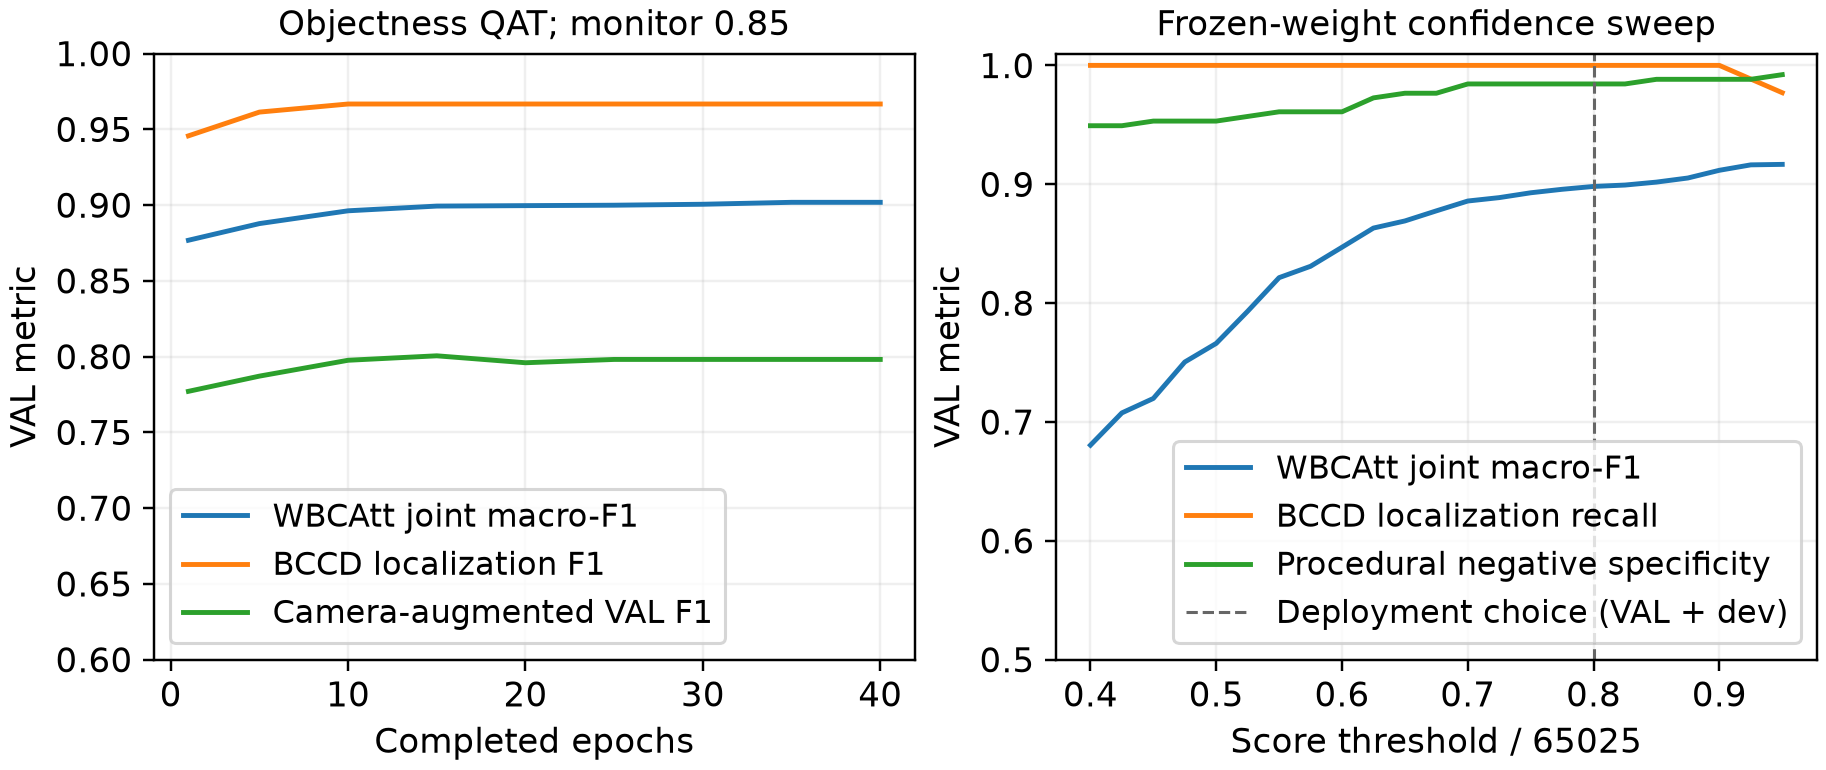
\includegraphics[width=0.98\linewidth]{images/two_source_training.png}
\captionof{figure}{仅objectness追加训练与开发阈值校准。左图固定0.85阈值监测，右图在冻结权重后扫描，虚线为结合公开验证及用户开发截图选定的部署阈值。程序空图特异性不是相机域性能。}
\end{center}



\begin{center}\small
\captionof{table}{截至2026年10月21日的验证与部署证据范围}
\begin{tabularx}{\linewidth}{|L{3.0cm}|Y|}
\hline\tablehead 类别 & 当前记录及适用范围\\\hline
模型与RTL & 冻结评估、向量和组件摘要通过；说明整数计算与调度一致\\\hline
资源与时序 & 最终候选完整主板物理摘要通过；本次未重新布局布线\\\hline
SRAM下载 & TD6.2成功摘要，候选bit哈希已核对\\\hline
Flash部署 & 本机自动操作失败；用户反馈手动完成，烧录文件身份未独立核验\\\hline
实拍与HDMI & 用户定性反馈实拍改善；定量精度、当前HDMI与冷启动待独立核验\\\hline
本次文档检查 & 核对活动RTL、模型/bit哈希与现存摘要；双遍编译并逐页检查PDF\\\hline
\end{tabularx}
\end{center}

\lead{运行状态与测量口径}
图像完整率表示一个视频帧所需的包是否全部收到，需结合 RAW 组数、输出像素数和累计流错误共同判断。FPGA 计时基准为 100 MHz，采集时间起点为帧首事件，不能直接等同于未知的光学曝光起点；PC 的拼帧时间使用单调时钟，上位机提交图像也不等同于显示面板发光时刻。

网络线速、DDR 带宽、CNN 周期和静态时序分别描述传输预算、存储访问、计算耗时和受约束路径裕量，不能直接相加替代从曝光到显示发光的实测延迟。本轮两来源模型已于2026年10月21日11:37通过TD6.2下载主板SRAM；随后收到用户实拍改善及手动Flash烧录完成的反馈。候选bit已核对SHA-256，但用户手动写入的Flash文件身份与断电冷启动未独立核验。本轮新位流SHA256为
\begin{center}\footnotesize
\texttt{5bc2dfee5ef0980b69b3749871bcd768298c5b37af3dcdb67af45930c8ceff58}
\end{center}
旧已验证bit和模型保持归档。本机自动Flash尝试在逐页编程/校验阶段后报\code{PRG-8000: get tdo buffer failed}，Tcl catch=1；该操作不记作成功。用户手动烧录反馈单独保留。后续需在带真值的相机场景记录误检、漏检、类别跳变、WAIT及响应时间；程序下载与用户定性反馈不能替代定量验收。\cite{twosource,programming}

\Needspace{12\baselineskip}
\section{总结}
\subsection{可扩展之处}
当前主工程已统一为\path{camera processing unit/}目录结构，主板采用WBCAtt+与BCCD两来源重训模型。SRAM下载已核实，用户反馈实拍改善并自行完成Flash烧录；手动烧录文件身份与冷启动尚未独立核验。此前单一来源新版因空场景误检撤回，历史证据保留。系统实现全帧量化联合检测分类、15 Hz抽帧、单框身份保持及英文全称。后续先采集主板相机带标签细胞数据，检查淋巴细胞弱项、照明与色彩偏差及小目标细节；再考虑输入分辨率、真正多尺度检测或多目标计数。剩余14块ERAM与5个DSP，扩大网络需综合吞吐、资源和时序。新增实时功能继续在板端实现。

\subsection{心得体会}
本项目的核心是把图像、时序和控制放在同一套可核对的数据约定下。RAW10 的组宽、有效行数、Bayer 相位、窗口中心和网络偏移都会影响最终画面的空间位置。只有在帧首、有效像素和坐标之间建立一致关系，算法模块才能在不改变主链路的条件下连接和复用。

自动图像调节同样需要明确反馈来源和执行时刻。AWB 应估计数字校正前的色偏，AE 应测量校正后亮度；曝光寄存器写入完成与图像反映新曝光之间存在延迟。控制器通过窗口平均、死区、限幅、积分管理和生效等待，把这些实际约束纳入硬件决策，参数提交则以帧边界保证整帧一致。

网络显示不是把 UDP 字节直接写进显存即可完成。包到达顺序、缺口填充、FIFO 门槛、DMA 突发和完整帧发布必须协同。数据从 DDR 返回时，采样基准应与 DQS 对应，跨域后的有效信号应描述真实收到的数据；进入 HDMI 前还需把 RGB 和同步信号延迟一致。这些约束共同决定图像是否在正确位置连续显示。

验证应覆盖接口两端和异常路径。像素参考模型用于核对数值，网络检查器用于核对线上格式，生产存储控制器和芯片模型用于核对读写关系，显示端逐像素比对用于核对最终光栅。功能仿真、静态时序和上板观察分别回答不同问题，将它们结合，才能形成可持续扩展的实时视觉系统。

检测分类接入表明，数据定义、预处理、量化和展示策略需要一起验证。WBCAtt+掩膜提供整细胞框和五类，BCCD只监督定位；去重与冲突剔除应在性能查看前固定。本轮权重由VAL选择，部署阈值另用开发截图校准，这些截图不能再作为独立验收。整数逐层对拍回答计算是否一致，完整视频仿真回答调度和结果保持是否正确，物理时序回答既有约束下能否运行。用户实拍改善反馈提供了定性证据，后续仍需独立带标签相机集、真实空场景统计与持续运行检查，才能量化公开数据结果在本板拍摄域中的表现。

\section{参考文献}
\begin{thebibliography}{99}
\setlength{\itemsep}{2pt}\raggedright
\bibitem{repo} 项目组. camera processing unit当前主工程与系统拓扑[CP]. 2026-10-21. 项目根目录\path{README.md}.
\bibitem{layout} 项目组. 工程目录映射与检查脚本[CP]. \path{tools/project_layout.json}, \path{tools/check_project_layout.py}. 历史构建路径按映射查找现存文件.
\bibitem{rtl} 项目组. 主板采集与ISP实现[CP]. \path{hardware/mainboard/user_source/hdl_source/}下\path{isp2/cvp_proc.v}及\path{isp2/cvp_demosaic.v}.
\bibitem{interface} 项目组. 公共像素流与结果接口[CP]. 同一RTL目录下\path{common/cvp_pixel_defs.vh}, \path{advanced/cvp_advanced.v}, \path{yolo/cvp_yolo_tracks.v}.
\bibitem{pid} 项目组. 定点PID、数字增益及帧统计[CP]. 同一RTL目录下\path{advanced/cvp_ae_control.v}, \path{advanced/cvp_gain11.v}, \path{advanced/cvp_frame_stats.v}；历史回归说明见\path{old/releases/v38-candidate/README.md}.
\bibitem{resource} 项目组. 当前两来源模型最终物理实现摘要[R]. TD 6.2.168116, 2026-10-21. \path{hardware/mainboard/reports/yolo_wbc_bccd15/current/physical/build_result.json}.
\bibitem{timing} 项目组. 主板构建与源码身份清单[R]. 同目录\path{source_hashes.json}及上级\path{summary.json}. 原始布线日志已清理，本文引用保留摘要.
\bibitem{hdmistart} 项目组. HDMI网络收流及显示架构说明[R]. \path{hardware/hdmi/doc/}下《架构文档\_网口收流HDMI输出.md》；\path{docs/design_notes/body_ch5.tex}.
\bibitem{hdmicolor} 项目组. 子板显示历史调试与验证说明[R]. \path{hardware/hdmi/doc/}下《handoff\_网口收流调试交接.md》；\path{docs/design_notes/body_ch5.tex}. 历史仿真结果不作为本次重跑结论.
\bibitem{gui} 项目组. 图像控制上位机[CP]. \path{hardware/mainboard/tools/cam_gui_v27.py}, \path{hardware/mainboard/tools/v27_client.py}.
\bibitem{yolortl} 项目组. 单尺度量化检测与板端集成实现[CP]. \path{yolo/model.py}；\path{hardware/mainboard/user_source/hdl_source/}下\path{yolo/}、\path{design_top_wrapper.v}及\path{classify/cvp_cell_label.v}.
\bibitem{yoloreport} 项目组. 15 Hz检测分类验证摘要[R]. \path{hardware/mainboard/reports/yolo_wbc_bccd15/current/summary.json}；同目录各\path{five_*/results.json}.
\bibitem{training} 项目组. 两来源冻结数据与模型审计[R]. \path{yolo/wbc_bccd/frozen/data_manifest.json}, \path{data_audit.json}, \path{protocol.json}, \path{test_regression.json}.
\bibitem{programming} 项目组. 主板部署与Flash操作摘要[R]. \path{hardware/mainboard/deployment_state.json}；\path{hardware/mainboard/reports/yolo_wbc_bccd15/}下\path{programming/programming.json}与\path{programming_flash_20261021/}.
\bibitem{wbcatt} TSUTSUI S, PANG W, HE S, et al. WBCAtt+: Fine-Grained Pixel-Level Morphological Annotations for White Blood Cell Images[J/OL]. Medical Image Analysis, 2026[2026-10-21]. \url{https://github.com/apple2373/wbcattplus}.
\bibitem{datarepo} TSUTSUI S, et al. WBCAtt+ Dataset[DS/OL]. Hugging Face, 2026[2026-10-21]. DOI:10.57967/hf/8143. \url{https://huggingface.co/datasets/apple2373/wbcattplus}. 下载与来源按本项目冻结数据清单记录.
\bibitem{twosource} 项目组. WBCAtt+与BCCD两来源训练及主板部署报告[R]. \path{docs/reports/}下《README\_1021\_WBCAtt与BCCD两来源重训.md》；\path{hardware/mainboard/reports/yolo_wbc_bccd15/README.md}；\path{yolo/wbc_bccd/frozen/}.
\bibitem{mechanical} 项目组. 显微镜摄像头支架V10结构设计与配合检查[R]. \path{MicroscopeSupport_V10/}设计包中的中文说明、\path{V10_Release.json}及\path{Fit_Verification.json}；装配模型与打印分件.
\bibitem{hdmiresource} 项目组. 子板HDMI工程发布与资源记录[R]. \path{old/releases/v28/README.md}. 占用率按记录的资源数量与总量计算.
\end{thebibliography}

\end{document}
